\begin{figure*}[t]
\centering
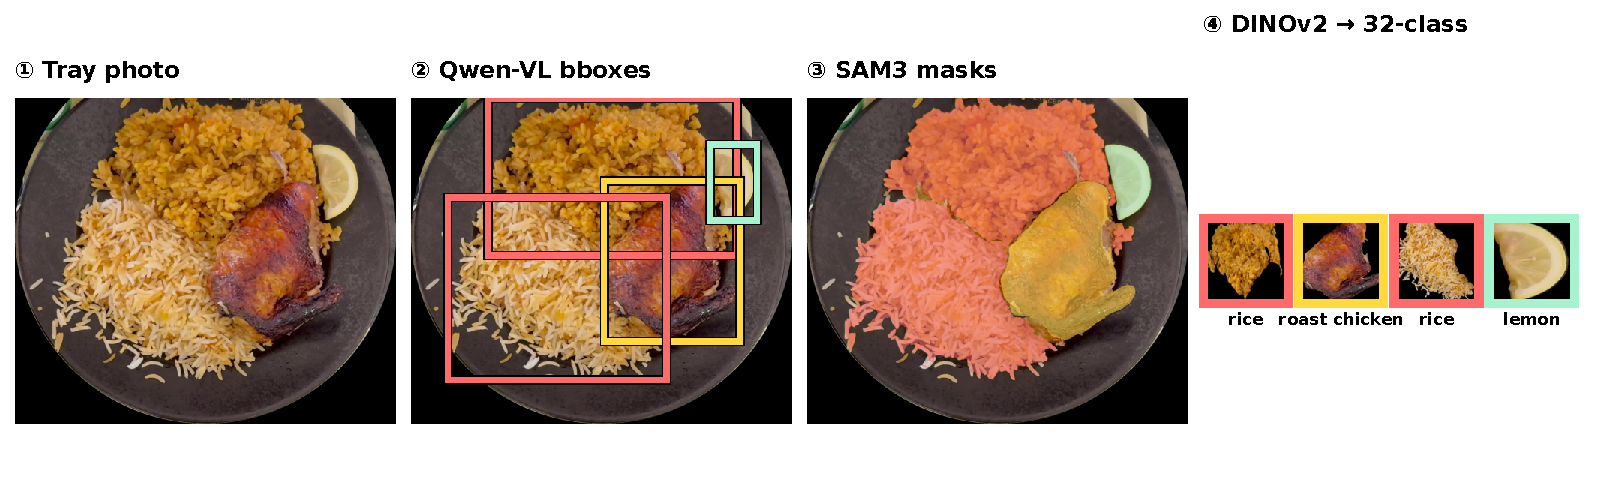
\includegraphics[width=\textwidth]{figs/pipeline_flow.pdf}
\caption{The teacher pipeline applied to a single tray. \textbf{(1)} Source
image. \textbf{(2)} Qwen2.5-VL-72B emits a JSON list of bounding boxes.
\textbf{(3)} SAM3 refines each bbox into a pixel mask. \textbf{(4)} Each masked
crop is embedded with DINOv2-large + SigLIP, clustered with HDBSCAN, and
collapsed by human curators into one of 32 dish classes. Here: rice, roast
chicken, rice (second helping), lemon. The student inference pipeline
(Figure~\ref{fig:pipeline-student}) follows the same flow at smaller scale.}
\label{fig:flow}
\end{figure*}

The teacher labeling pipeline is itself a three-stage cascade, run \emph{once}
on a curated 4{,}999-image subset of cafeteria tray photos. The output is a
labeled training set; no part of this pipeline runs at inference time.
Figure~\ref{fig:pipeline-teacher} shows the full architecture --- note the
deliberate symmetry with the student pipeline (Figure~\ref{fig:pipeline-student}):
the same three-stage decomposition, with frozen 72B / DINOv2+SigLIP /
HDBSCAN at the labeling scale and fine-tuned 7B / SAM3 / DINOv2 $k$-NN at
the inference scale.

\begin{figure}[t]
\centering
\begin{tikzpicture}[
  node distance=4pt and 6pt,
  every node/.style={font=\footnotesize},
  stage/.style={rectangle, draw=black, rounded corners=2pt, minimum width=1.55cm,
                minimum height=0.8cm, align=center, fill=orange!15},
  artifact/.style={rectangle, draw=gray!60, rounded corners=1pt, minimum height=0.55cm,
                   align=center, fill=gray!8, font=\scriptsize},
  arrow/.style={-{Latex[length=2mm]}, thick}
]
  \node[artifact]              (raw)   {4{,}999 raw\\tray images};
  \node[stage, right=of raw]   (vlm)   {\textbf{Stage 1}\\Qwen2.5-VL\\72B-AWQ\\(frozen)};
  \node[stage, right=of vlm]   (sam)   {\textbf{Stage 2}\\SAM3\\(frozen)};
  \node[stage, right=of sam]   (clu)   {\textbf{Stage 3}\\DINOv2 +\\SigLIP +\\HDBSCAN};
  \node[artifact, right=of clu, text width=1.65cm] (out)
        {\textbf{v3.2}\\4{,}629 items\\32 classes};
  \draw[arrow] (raw) -- (vlm);
  \draw[arrow] (vlm) -- node[above]{\scriptsize bbox+name} (sam);
  \draw[arrow] (sam) -- node[above]{\scriptsize masks} (clu);
  \draw[arrow] (clu) -- node[above, align=center]{\scriptsize human\\curate} (out);
\end{tikzpicture}
\caption{Teacher labeling pipeline. A 72B vision-language model emits
structured-JSON detections; SAM3 refines bboxes into masks; DINOv2 + SigLIP
embeddings drive HDBSCAN clustering and are then collapsed to a 32-class
ontology by human curators. The pipeline runs once offline. Compare
Figure~\ref{fig:pipeline-student}: the student inference pipeline mirrors
this architecture at $\sim$10$\times$ smaller scale.}
\label{fig:pipeline-teacher}
\end{figure}

\subsection{Stage 1 (Teacher VLM): Qwen2.5-VL-72B-AWQ}
\label{sec:de:vlm}

The first stage is a 72B-parameter vision-language model
(\texttt{Qwen/Qwen2.5-VL-72B-Instruct-AWQ}) served via vLLM with FP8 KV-cache
and prefix caching. It is prompted to emit a strict JSON list of
\texttt{name}, \texttt{description}, and \texttt{bbox} per visible food region,
with explicit \emph{splitting rules} (mixed dishes are one item, toppings stay
with their base dish) and \emph{exclusion rules} (no plates, trays, utensils,
empty containers, or labels). The full prompt --- which encodes much of the
dataset's ontology --- is reproduced in Figure~\ref{fig:prompt-template}.

\begin{figure}[t]
\centering
\fbox{\parbox{0.95\columnwidth}{\footnotesize\ttfamily
You are analyzing a cafeteria tray. Find EVERY food and beverage item --- do
not miss anything. Scan the full image carefully: main dishes, sides, bread,
dips, drinks, juice boxes, yogurt cups, fruit, desserts.
\\[2pt]
For each item return:
\\[1pt]
\textendash\ \textbf{name}: short common name (e.g.\ ``kabsa rice'')
\\
\textendash\ \textbf{description}: visual texture ONLY; no plates/positions
\\
\textendash\ \textbf{bbox}: \texttt{[x1, y1, x2, y2]} absolute pixels
\\[2pt]
\textbf{Splitting rules:}
\\
\textendash\ Different foods $=$ separate items
\\
\textendash\ Same food in two places $=$ list twice
\\
\textendash\ A topping is part of its base dish (oil on hummus $=$ one item)
\\
\textendash\ A mixed dish (stew, salad) $=$ one item
}}
\caption{Stage~1 prompt for the Qwen2.5-VL-72B teacher. The splitting rules
encode the dataset's ontology. \emph{Toppings stay with their base} is the
single most important constraint --- it is what distinguishes ``rice with sauce''
(one item) from ``rice and sauce'' (two items) for billing purposes.}
\label{fig:prompt-template}
\end{figure}

The 72B teacher succeeds on 4{,}999 / 4{,}999 images (zero JSON-parse failures)
in 5{,}778~s of wall-clock time (roughly $1.16$~s/image at the AWQ-quantised
weight precision).

\subsection{Stage 2 (Teacher SAM): SAM3 mask refinement}
\label{sec:de:sam}

For each VLM-emitted bbox, SAM3 is prompted with the box and produces a
pixel-accurate mask. We apply a confidence cascade
($0.10 \rightarrow 0.05 \rightarrow 0.02 \rightarrow 0.01$) so that
low-contrast items are not silently dropped, and a global mask-IoU NMS at
$0.7$ to suppress duplicate masks within the same image. SAM3 succeeds on
$4{,}948$ / $4{,}999$ images; the $51$ failures (1.0\%) are primarily very
small or very low-contrast regions and are excluded from training rather than
heuristically recovered.

\subsection{Stage 3 (Teacher classifier): cluster + curate}
\label{sec:de:cluster}

The 72B teacher's open-vocabulary names (e.g.\ ``cheesecake slice'',
``chocolate cake'', ``yellow cake'') need to be collapsed into a closed
taxonomy for downstream training. Each masked crop is embedded with frozen
DINOv2-large (1024-d vision) and SigLIP (768-d, fused via the VLM's
\texttt{name} string), reduced via UMAP, and clustered with HDBSCAN. The
result is $467$ raw clusters, of which $1{,}744$ items are labeled noise.
Human curators inspect cluster centroids in an interactive viewer
(\texttt{dataset\_inspect/}) and (i)~merge near-synonymous clusters
(``cheesecake slice'' + ``chocolate cake'' + ``fruit tart'' $\rightarrow$
\textbf{cake}), (ii)~drop clusters that are not edible (e.g.\ utensil
artifacts), and (iii)~recover the highest-confidence noise items into the
nearest valid cluster (the \texttt{noise\_recovery} step in v3.1, surfacing
$1{,}344$ recovered items).

\subsection{Final dataset (v3.2)}
\label{sec:de:final}

The released v3.2 export filters to images where every 72B-detected region
survives SAM3 and clustering (i.e., complete labels per image). It contains
\textbf{4{,}629 items across 2{,}981 unique images and 32 classes}, with an
average of $1.55$ items per image. Class frequency is heavily long-tailed
(Figure~\ref{fig:class-dist}): \texttt{rice} alone accounts for $32\%$ of all
items, while five tail classes have fewer than $10$ items each.
Items are partitioned into train/dev/test ($80/10/10$, image-level
stratified, seed $420$) before any model training.

\begin{figure}[t]
\centering
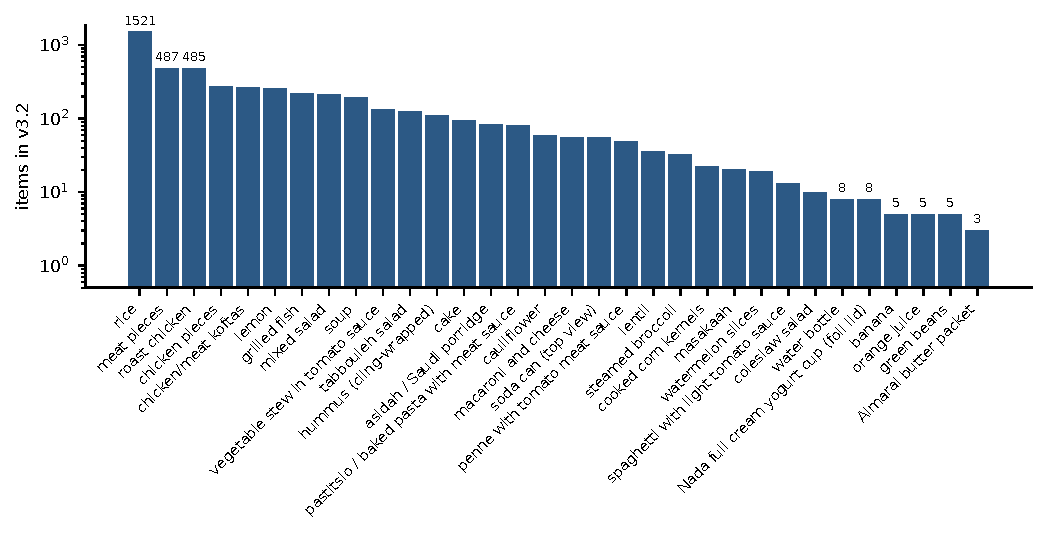
\includegraphics[width=\columnwidth]{figs/class_distribution.pdf}
\caption{Per-class item counts in the v3.2 training set, sorted descending.
The distribution is heavily long-tailed: top-3 classes account for over half
of all items; five tail classes have fewer than ten items each.}
\label{fig:class-dist}
\end{figure}

\begin{table}[t]
\centering\small
\begin{tabular}{l r}
\toprule
Source images (deduplicated)         & 4{,}999 \\
72B-VLM successful detections        & 4{,}999 (100.0\%) \\
SAM3 successful segmentations        & 4{,}948 (99.0\%) \\
Wall-clock teacher run-time          & 5{,}778~s ($\approx$96~min) \\
Raw HDBSCAN clusters                 & 467 \\
Noise items (HDBSCAN)                & 1{,}744 \\
Final classes (post-curation)        & 32 \\
Final items                          & 4{,}629 \\
Final unique images                  & 2{,}981 \\
\bottomrule
\end{tabular}
\caption{Teacher pipeline scale and yield.}
\label{tab:de:scale}
\end{table}

\subsection{Class taxonomy and distribution}
\label{sec:de:taxonomy}

The $32$-class final ontology was reached by collapsing the $467$ raw
HDBSCAN clusters along three axes: (i)~visual synonymy (different
cheesecake variants $\rightarrow$ \texttt{cake}); (ii)~price equivalence
under the cafeteria's billing rules (\texttt{rice} subsumes plain rice,
kabsa rice, mandi rice, biryani because they bill identically); and
(iii)~sub-cluster artefact removal (utensil-only or empty-plate clusters
were dropped). Table~\ref{tab:de:classes} lists all 32 classes with their
v3.2 item counts; the distribution is heavily long-tailed (top class
contains $32\%$ of all items, $5$ tail classes have fewer than $10$
items each).

\begin{table}[t]
\centering\scriptsize
\setlength{\tabcolsep}{4pt}
\begin{tabular}{lr|lr}
\toprule
\textbf{Class}                                  & \textbf{n} & \textbf{Class}                                & \textbf{n} \\
\midrule
rice                                            & 1521 & cake                                          & 95   \\
roast chicken                                   & 530  & hummus (cling-wrapped)                        & 110  \\
meat pieces                                     & 515  & pastitsio / baked pasta with meat sauce       & 81   \\
chicken pieces                                  & 268  & macaroni and cheese                           & 56   \\
lemon                                           & 240  & lentil                                        & 53   \\
mixed salad                                     & 210  & penne with tomato meat sauce                  & 49   \\
soup                                            & 197  & soda can (top view)                           & 55   \\
vegetable stew in tomato sauce                  & 132  & steamed broccoli                              & 45   \\
grilled fish                                    & 219  & cauliflower                                   & 32   \\
chicken/meat koftas                             & 113  & cooked corn kernels                           & 22   \\
tabbouleh salad                                 & 125  & masakaah                                      & 17   \\
asidah / Saudi porridge                         & 86   & watermelon slices                             & 16   \\
\midrule
spaghetti with light tomato sauce               & 11   & coleslaw salad                                & 8    \\
Nada full cream yogurt cup (foil lid)           & 7    & Almarai butter packet                         & 1    \\
green beans                                     & 1    & water bottle                                  & 1    \\
orange juice                                    & 1    & --- & --- \\
\bottomrule
\end{tabular}
\caption{All 32 v3.2 classes with item counts. The lower 6 rows hold the
visible long-tail (single-digit support each); these classes are
preserved in the dataset for completeness but our evaluation is
conservative on them, and we flag any per-class result with $n\!<\!10$
test instances as advisory only. The class names retain their original
descriptors (e.g.\ ``Almarai butter packet'') because billing requires
the brand-specific SKU.}
\label{tab:de:classes}
\end{table}

\subsection{Quality control and curator workflow}
\label{sec:de:curation}

Cluster curation was performed in an interactive HTML viewer
(\texttt{dataset\_inspect/cluster\_viewer.html}) that surfaces, for each
of the 467 raw clusters, (i)~the $16$ closest crops to the cluster
centroid in DINOv2+SigLIP joint space, (ii)~the union of VLM-emitted
class names within the cluster, and (iii)~a free-text \texttt{display\_name}
input. A single curator labeled all $467$ clusters in $\approx 4$
hours, with a second pass to merge near-duplicate clusters (e.g.\
\texttt{rice} appearing as 8 small clusters because the 72B teacher
emitted slight name variants). Boundary clusters --- those with
ambiguous content or visible mis-labeling --- were resolved by inspecting
$10$ random crops outside the centroid neighbourhood; if the cluster
was genuinely heterogeneous it was split, otherwise the dominant label
was applied.

The HDBSCAN noise bin (originally $1{,}744$ items, $\approx 35\%$ of
the post-SAM yield) was processed by a separate \emph{noise recovery}
pass that re-embedded each noise item, computed cosine similarity to
each curated cluster's centroid, and assigned it to the nearest cluster
if the similarity exceeded $0.75$. This recovered $1{,}344$ items
($77\%$ of noise) at the price of one parameter ($0.75$). Items that
remained in the noise bin were dropped from v3.2 entirely. Per-cluster
recovery threshold tuning is in scope for v3.3.
